\documentclass[14pt]{beamer}
\title[CP01.13 BC]{COJ :: Getting Started With Java}
\author[TS]{TalentSprint}
\institute[L\&D]{Licensed To Skill}
\date{Version 1.0.4}
\usefonttheme{serif}
\usecolortheme{orchid}
\usepackage{bookman}
\usepackage{hyperref}
\usepackage[T1]{fontenc}
\usepackage{graphicx}
\graphicspath{{../../Images/}}
\beamertemplateballitem
\usebackgroundtemplate{
\includegraphics[width=\paperwidth]{TS-Logo.jpg}}

\begin{document}
\begin{frame}
  \titlepage
\end{frame}
\begin{frame}{OO Thinking}
The content in this presentation is aimed at teaching  learners to
 \begin{itemize}
  \item Identify various concepts of OOPs
  \item Relate Object-Oriented approach to the process of understanding and analyzing complex systems in the real world.
 \end{itemize}
\end{frame}
\begin{frame}{OO Thinking}

Module Snapshot
\begin{center}
    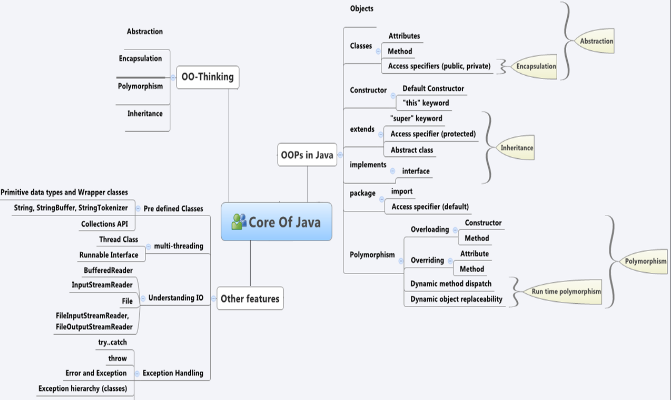
\includegraphics[scale=0.4]{ModuleSnapShot.png}
  \end{center}
\end{frame}

\begin{frame}{OO Thinking}
\begin{center}
    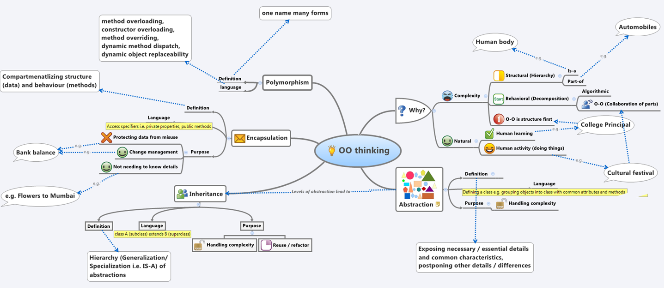
\includegraphics[scale=0.4]{Image2.png}
  \end{center}
\end{frame}

\begin{frame}{OO Thinking}
OOPs in Java
\begin{center}
    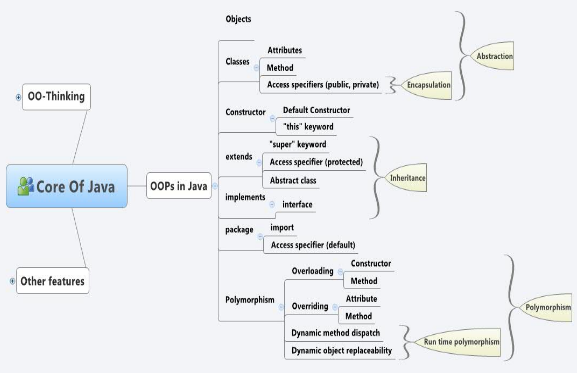
\includegraphics[scale=0.5]{Image3.png}
  \end{center}
\end{frame}

\begin{frame}{OO Thinking}
Why OO thinking?
\begin{center}
    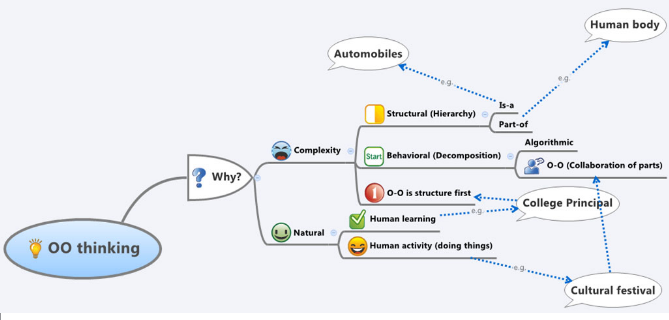
\includegraphics[scale=0.5]{Image4.png}
  \end{center}
\end{frame}

\begin{frame}{OO Thinking}
\begin{block}{}
  Dealing with complexity   
 \end{block}
\begin{itemize}
\item Complexity can be in structure as well as behavior.
\item The structure of complex systems is Hierarchic, - IS A hierarchy and part of hierarchy.
\item Behavioral complexity can be handled by collaboration of its parts.
 \end{itemize}
 \end{frame}
\begin{frame}{OO Thinking}
Structural Complexity
\begin{center}
    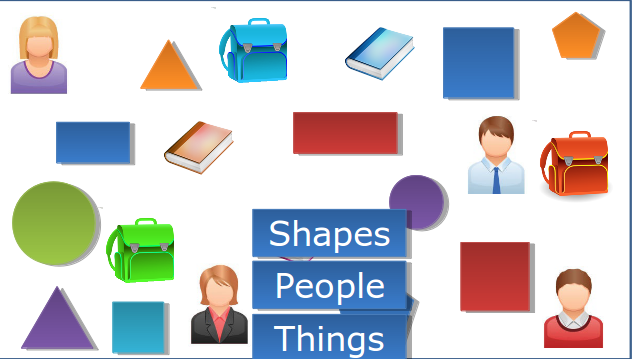
\includegraphics[scale=0.5]{Image5.png}
\end{center}
\end{frame}
\begin{frame}{OO Thinking}
Structural Complexity
\begin{center}
    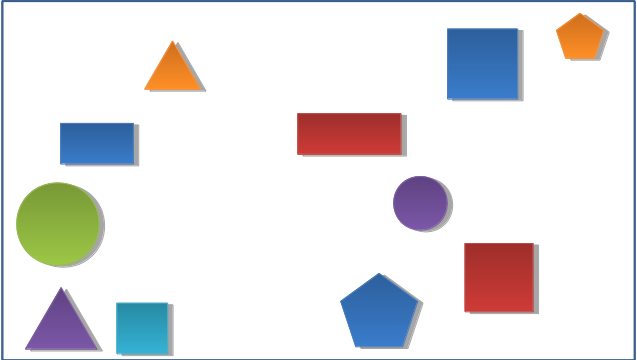
\includegraphics[scale=0.5]{Image6.png}
\end{center}
\end{frame}
\begin{frame}{OO Thinking}
Structural Complexity
\begin{center}
    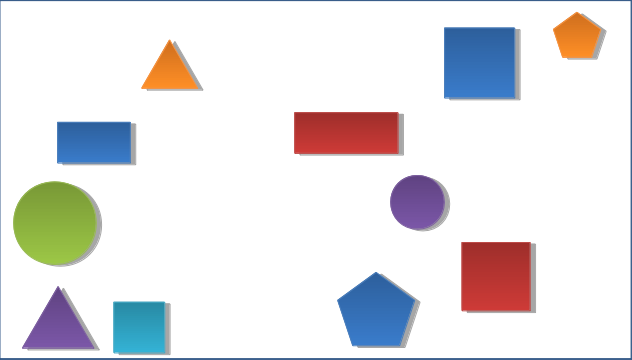
\includegraphics[scale=0.5]{Image7.png}
\end{center}
\end{frame}
\begin{frame}{OO Thinking}
Abstraction
\begin{center}
    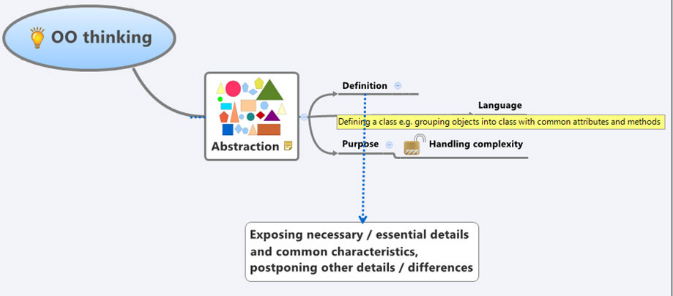
\includegraphics[scale=0.5]{Image8.png}
\end{center}
\end{frame}
\begin{frame}{OO Thinking}
Abstraction
\begin{center}
    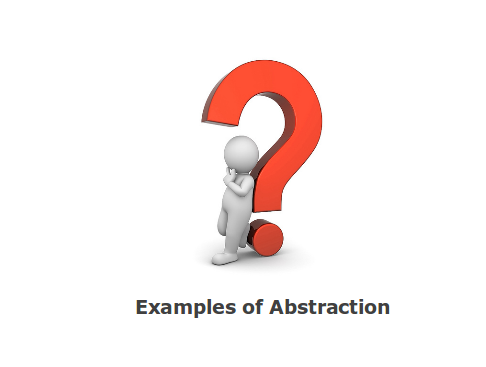
\includegraphics[scale=0.5]{Image9.png}
\end{center}
\end{frame}
\begin{frame}{OO Thinking}
Examples of Abstraction : Student
\begin{center}
    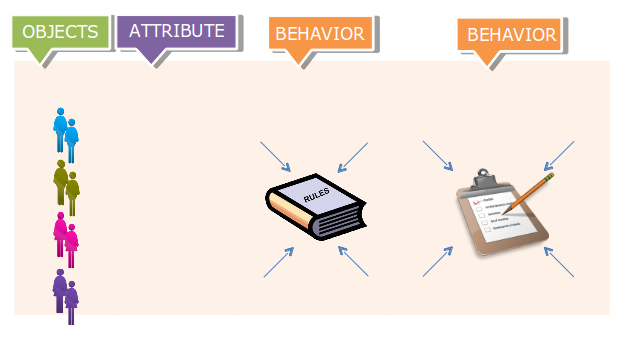
\includegraphics[scale=0.5]{Image10.png}
\end{center}
\end{frame}
\begin{frame}{OO Thinking}
Examples of Abstraction : Manufacturing of Automobiles
\begin{center}
    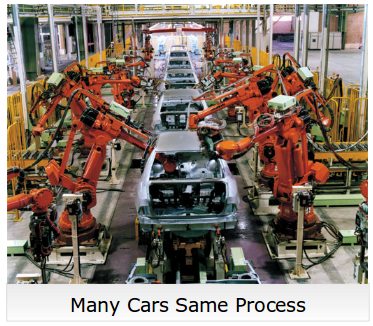
\includegraphics[scale=0.5]{Image11.png}
\end{center}
\end{frame}
\begin{frame}{OO Thinking}
Other definitions of Abstraction:

\begin{tabular}{l l}
\begin{minipage}{0.25\textwidth}
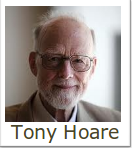
\includegraphics[scale=.6]{Image12.png}
\end{minipage}
&
\begin{minipage}{0.65\textwidth}
``Abstraction arises from a recognition of similarities between certain objects, situations, or processes in the real world, and the decision to concentrate upon those similarities and to ignore for the time being the differences.''
\end{minipage}
\end{tabular}
\end{frame}

\begin{frame}{OO Thinking}
Other definitions of Abstraction:
\begin{tabular}{l l}
\begin{minipage}{0.25\textwidth}
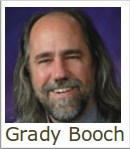
\includegraphics[scale=.6]{Image13.png}
\end{minipage}
&
\begin{minipage}{0.65\textwidth}
``An abstraction denotes the essential characteristics of an object that distinguish it from all other kinds of objects and thus provide crisply defined conceptual boundaries, relative to the perspective of the viewer.''
\end{minipage}
\end{tabular}
\end{frame}
\begin{frame}{OO Thinking}
Inheritance
\begin{center}
    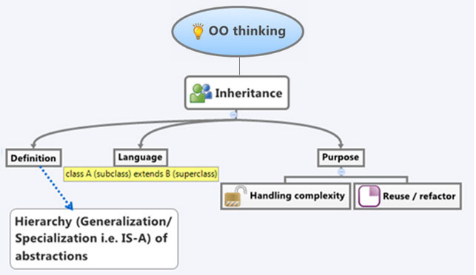
\includegraphics[scale=0.5]{Image14.png}
\end{center}
\end{frame}
\begin{frame}{OO Thinking}
IS-A Hierarchy
\begin{center}
    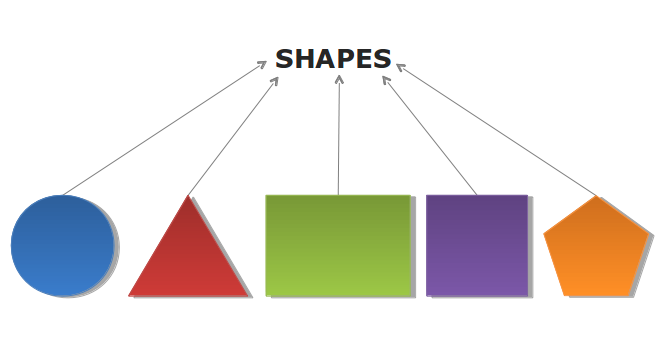
\includegraphics[scale=0.5]{Image15.png}
\end{center}
\end{frame}
\begin{frame}{OO Thinking}
Inheritance Example : Doctor
\begin{center}
    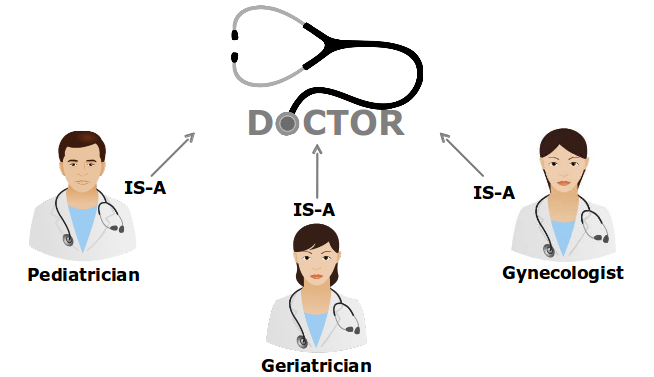
\includegraphics[scale=0.5]{Image16.png}
\end{center}
\end{frame}
\begin{frame}{OO Thinking}
Inheritance Example: Car
\begin{center}
    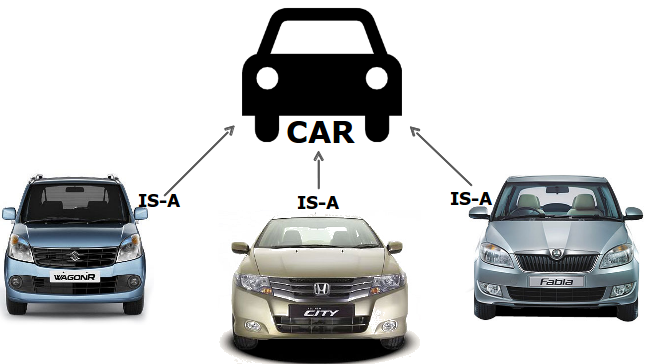
\includegraphics[scale=0.5]{Image17.png}
\end{center}
\end{frame}
\begin{frame}{OO Thinking}
Inheritance Example: Student
\begin{center}
    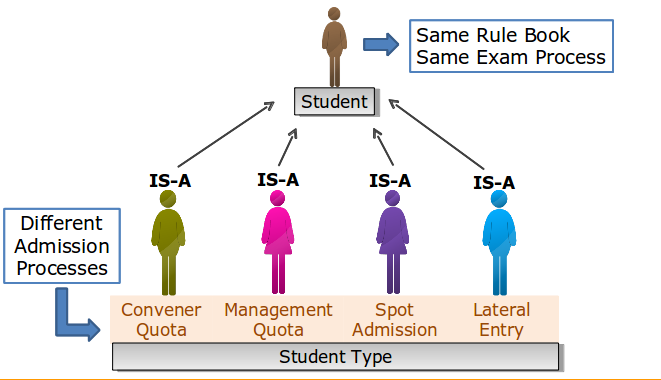
\includegraphics[scale=0.5]{Image18.png}
\end{center}
\end{frame}
\begin{frame}{OO Thinking}
Encapsulation
\begin{center}
    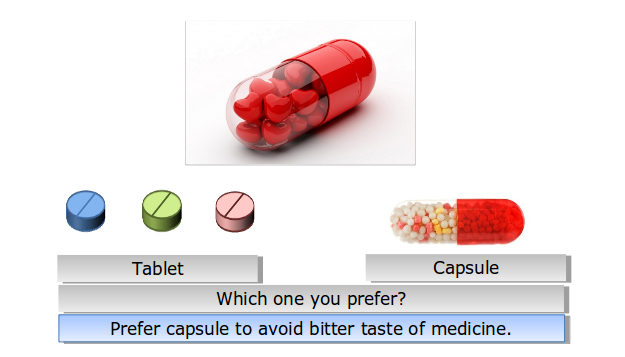
\includegraphics[scale=0.5]{Image19.png}
\end{center}
\end{frame}
\begin{frame}{OO Thinking}
Encapsulation
\begin{center}
    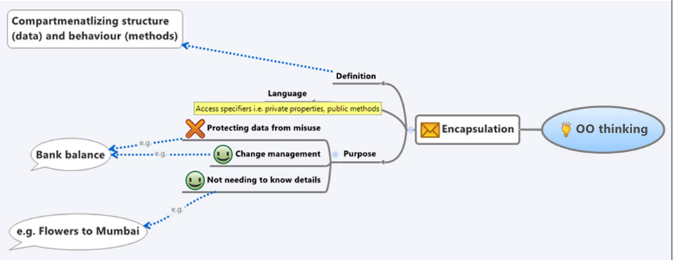
\includegraphics[scale=0.5]{Image20.png}
\end{center}
\end{frame}
\begin{frame}{OO Thinking}
Encapsulation Example: Bouquet to Delhi 
\begin{center}
    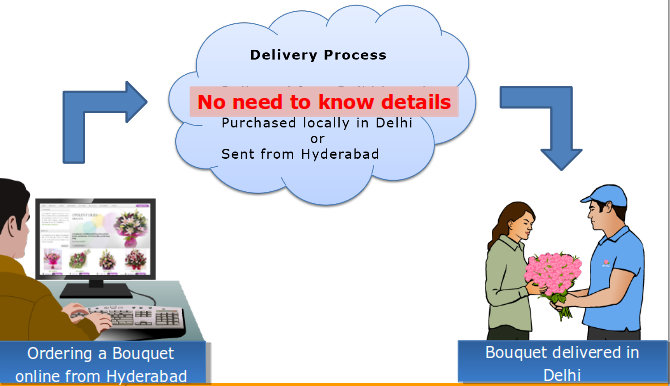
\includegraphics[scale=0.5]{Image21.png}
\end{center}
\end{frame}
\begin{frame}{OO Thinking}
Encapsulation Example: Bank Account Balance
\begin{center}
    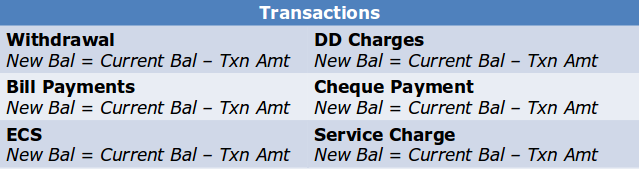
\includegraphics[scale=0.5]{Image22.png}
\end{center}
\end{frame}
\begin{frame}{OO Thinking}
Encapsulation Example: Bank Account Balance
\begin{center}
    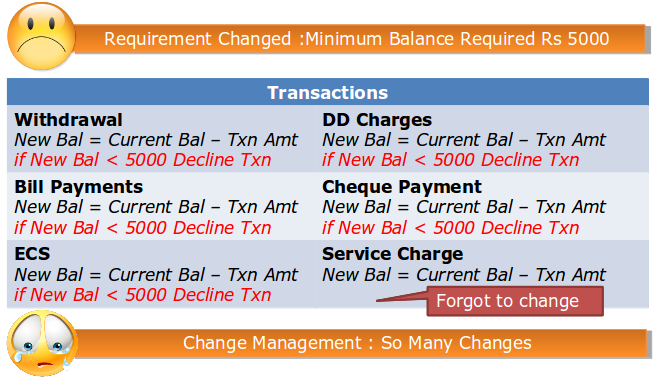
\includegraphics[scale=0.5]{Image23.png}
\end{center}
\end{frame}
\begin{frame}{OO Thinking}
Encapsulation Example: Bank Account Balance
\begin{center}
    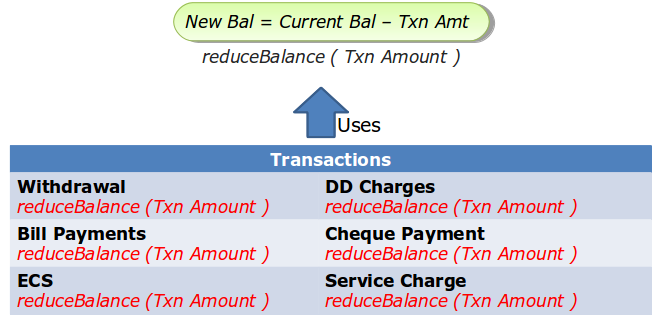
\includegraphics[scale=0.4]{Image24.png}
\end{center}
\end{frame}
\begin{frame}{OO Thinking}
Encapsulation Example: Bank Account Balance
\begin{center}
    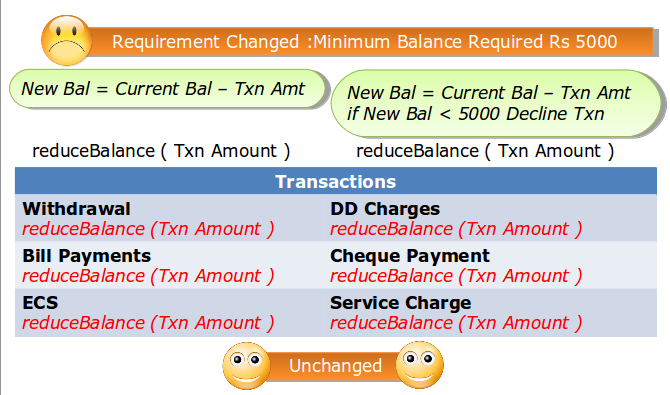
\includegraphics[scale=0.4]{Image28.png}
\end{center}
\end{frame}
\begin{frame}{OO Thinking}
Encapsulation Example: Catering
\begin{center}
    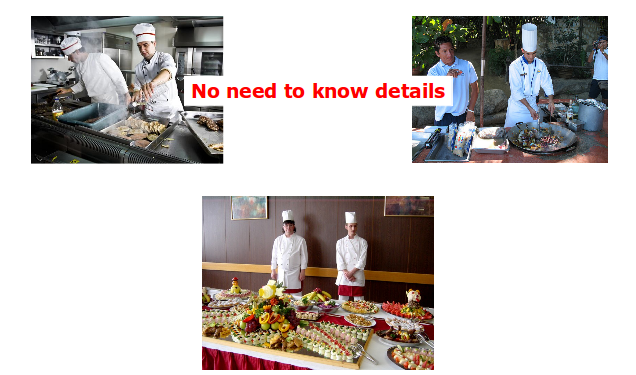
\includegraphics[scale=0.5]{Image25.png}
\end{center}
\end{frame}
\begin{frame}{OO Thinking}
Polymorphism
\begin{center}
    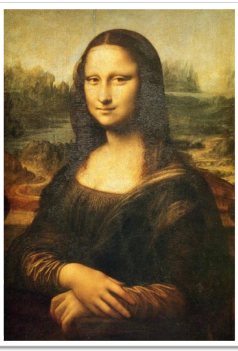
\includegraphics[scale=0.5]{Image26.png}
\end{center}
\end{frame}
\begin{frame}{OO Thinking}
Polymorphism
\begin{center}
    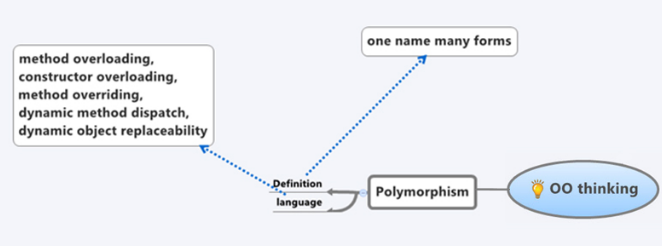
\includegraphics[scale=0.5]{Image27.png}
\end{center}
\end{frame}
\begin{frame}{OO Thinking}

\begin{center}
    
\includegraphics[scale=0.5]{Image29.png}
\end{center}
\end{frame}
\end{document}

